\section{Data Acquisition}
\label{section:data}

%The data acquisition component of \textit{GESTALT} begins with a visual and geospatial encoding of the world. 
%The visual encoding is primarily remote sensing imagery providing a top-down view of the earth's surface, but it also includes street-view imagery and other photographs. 
\emph{GESTALT} enables last-mile search by encoding visual and geospatial data within a given \emph{region}, using two types of geotags: \emph{object} tags and \emph{location} tags.

\textbf{\emph{Regions}} represent a limited physical area of interest within which a last-mile search will be performed. 
Regions can be arbitrary and represent an administrative boundary like a city, suburb, or general geographic area.
Regions are defined by bounding boxes for compatibility with the OSM and Flickr APIs.

\textbf{\emph{Objects}} represent any physical entity located within the region of interest. 
For example, a \textit{tree, building, lake, bridge, gate} or \textit{sign} could be an object. 
\textit{Objects} can also have attributes that provide amplifying information about them, including things like \textit{color, material, size, species, etc.}. 

\textbf{\emph{Locations}} represent physical entities that \textit{do} something, giving them a purpose beyond that of objects. 
Locations can contain meaningful groupings of objects determined by ownership, proximity, or utility. 
Examples of locations include \textit{businesses, attractions, properties, etc.}. 
\textit{Locations} have \textit{objects} associated with them, and \emph{GESTALT} enables users to query for locations given a partial set of knowledge about the objects at those locations.

\subsection{Object Tags}
To maximize dataset coverage and demonstrate the flexibility of \emph{GESTALT}, we support three methods of ingesting objects:
\begin{enumerate}
    \item Ingesting KML Files that contain manually annotated objects and their coordinates.
    \item Querying the Open Street Maps (OSM) API to ingest crowd-sourced object tags and their coordinates.
    \item Automatically detecting objects in geolocated photos pulled from the Flickr API. 
\end{enumerate}

Upon ingest, each object is assigned a confidence score, reflecting the certainty that the object tagged at those coordinates exists and is of the type annotated. 
For results reported in this paper, we adopt the rule that hand-labeled objects receive a confidence score of $1.0$, OSM objects receive a score of $0.75$, and objects labeled by the object detector receive the confidence score reported by the object detection model. Table~\ref{table:DataSet} contains a summary of the objects currently in \emph{GESTALT}.

\subsection{Location Tags}
We support two methods of ingesting locations:
\begin{enumerate}
    \item Ingesting KML Files that contain manually annotated locations and their coordinates.
    \item Querying the Open Street Maps (OSM) API to ingest crowd-sourced location tags and their coordinates. 
\end{enumerate}

Similar to the approach with object tags, we assign a confidence to each location tag ingested based on the source providing it.



\begin{figure}[h!]       
    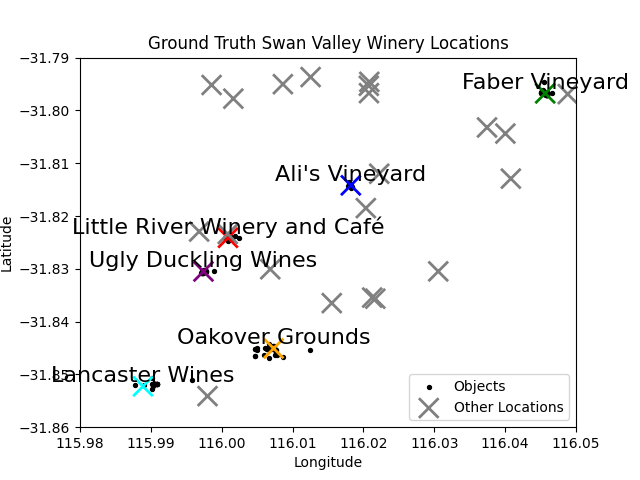
\includegraphics[width=0.5\textwidth]{loc_labels_plot.png}
    %\centering
    \caption{The Swan Valley Wineries dataset has six locations with annotated objects and another 30 without manually annotated objects but with confirmed location coordinates.}
    \label{fig:loc} 
\end{figure}


\subsection{Ingest Methods}
\subsubsection{Ground Truth Hand Labeled Tags} 
Hand-labeled objects and locations have been manually annotated by a trustworthy source and are assumed to be correctly labeled and geotagged. 
\emph{GESTALT} accepts hand-labeled tags to allow for prior manual annotation work to be folded into the pipeline and to provide a reliable means to report results on ground truth data so that we can compare \emph{GESTALT} with future architectures that might attempt to solve the last-mile search problem with a different approach. 
For benchmarking purposes, we curated the \emph{Swan Valley Wineries} dataset containing 31 ground truth location tags for wineries (and five for breweries) in the Swan Valley Region of Western Australia and 146 ground truth object tags associated with six of those wineries. 

The wineries dataset tags are stored in Keyhole Markup Language~\footnote{\href{https://developers.google.com/kml/documentation/kml\_tut}{https://developers.google.com/kml/documentation/kml\_tut}} (KML).
The tags consist of an object name, its latitude \& longitude, and any descriptive markings written as key:value pairs. 

The object tagging was conducted manually by a single annotator using \textit{Google Earth Professional \footnote{\href{https://www.google.com/earth/about/versions/}{https://www.google.com/earth/about/versions/}} version 7.3}. 
The data sources include on-the-ground knowledge, manual inspection of satellite imagery, street-view imagery, and publicly available area photos. 
The objects tagged are representative, not exhaustive. 
Attributes of the objects (e.g., color, size, material) are recorded in the comments field as key:value pairs.
Each object from the hand-labeled dataset is assigned a confidence score of 1.0 since it was manually identified and tagged.
The object tags are aligned with their corresponding winery location in the dataset.
Figure \ref{fig:loc} shows the winery locations in the Swan Valley Wineries dataset, and Figure \ref{fig:loc-obj} shows each of the six wineries that was hand labeled with ground-truth object tags, along with those tags and their spatial locations with respect to the winery location.


\begin{figure*}[ht]
    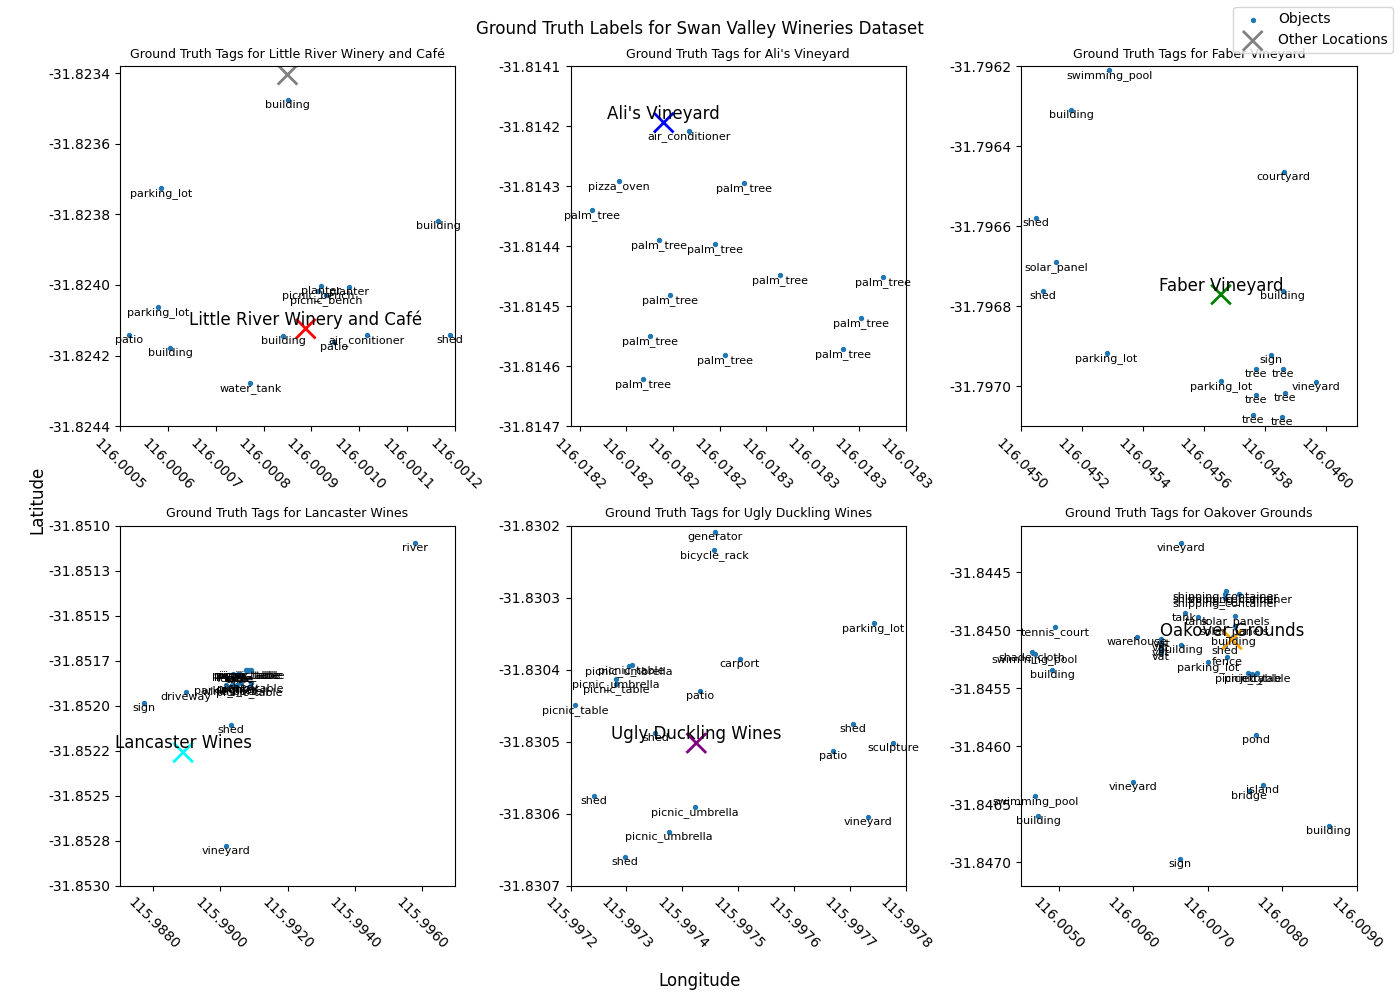
\includegraphics[width=\textwidth]{loc_obj_labels_plot.png}
    \centering
    \caption[width=\textwidth]{A representative view of the six wineries in the dataset shows the geospatial heterogeneity of object positions between locations.}
    \label{fig:loc-obj}  
\end{figure*}


\subsubsection{Open Street Maps Tags}
\osullikomment{I think we can afford to trim this section down if we need the space}
\emph{GESTALT} can also ingest object and location tags by querying the Open Street Maps (OSM) API.
OSM is a knowledge collective that contains open-source Geodata~\cite{Haklay2008}, in the form of  \textit{elements}\footnote{\href{https://wiki.openstreetmap.org/wiki/Elements}{https://wiki.openstreetmap.org/wiki/Elements}}. 
The key element subtypes are \textit{Nodes} (point data for objects and locations) \textit{ways} (line data for roads, creeks, railways, etc.) and \textit{relations} (for relationships between elements, like suburb-state).
While businesses, attractions, and other \textit{locations} are commonly annotated by the OSM community, \textit{objects} are more sparsely tagged as they are typically less interesting subject matter. 
\emph{GESTALT} ingests \textit{nodes} through the Overpass API using the OSMPythonTools package \footnote{\href{https://pypi.org/project/OSMPythonTools/}{https://pypi.org/project/OSMPythonTools/}}, pulling all nodes within a given bounding box that have at least one tag (like "name," "craft," etc.).
The initial list of nodes is pruned to remove results not likely referring to objects or that lack detail to be resolved to objects.
The remaining nodes are transformed into a standard JSON format and stored for indexing and search later in the \emph{GESTALT} pipeline. 

Businesses, attractions, and other higher-level \textit{locations} are commonly annotated as nodes in OSM by the open-source community or business owners. 
We retrieve them from the OSM Overpass API similarly to objects, but this time excluding results that lack features like names, street addresses, and phone numbers. 
We assign each location or object tag ingested from OSM is assigned a confidence score of 0.75 because while any user can edit tags in the OSM database without review, the open-source community does have some degree of self-regulation~\cite{VargasMunoz2020}, and prior work has examined the application of machine learning for detecting anomalous behavior in OSM edits~\cite{Mooney2017}.
While OSM provides a rich, free, and accessible data source to leverage the power of the crowds to generate tags for \emph{GESTALT}, the completeness of OSM is generally unassured, so scaling \textit{GESTALT} beyond the trivial requires an automated method for object detection and resolution. 

\subsubsection{Noisy Image-based Tags}
The third and most important method by which \emph{GESTALT} ingests objects is through automatic object detection.
We query the Flickr API for images uploaded within a given region (bounding box) since January 1$^{st}$ 2020. 
Given those images and their EXIF metadata, the Object Detection module uses pre-trained YOLO v.8~\footnote{\href{https://github.com/ultralytics/ultralytics}{YOLO}} to identify objects in each image from 80 classes (based on the COCO dataset~\footnote{\href{{https://cocodataset.org/}}{https://cocodataset.org/}}). 
Those objects become tags in \emph{GESTALT}, with their coordinates determined by the geolocation of the image and their confidence score determined by YOLO's confidence at the detection step.
For our experiments we enable safe-search and limit to public photos that have been added since January 1$^st$ 2020. For the Swan Valley Region we retrieve 462 images, and for the Washington DC Region, we pull a representative 4,000 images out of over 12,000 available. 

\small{
\begin{table}[h!]
    \begin{center}
        \begin{tabular}{ |c|c|c|c|c| } 
            \hline
            Dataset & Source & Ingest Method & \# Tags \\%& \# Unique \\
            \hline
            \multirow{5}{8em}{Swan Valley Wineries\tablefootnote{BoundingBox:['115.96168231510637', '-31.90009882641578', '116.05029961853784', '-31.77307863942101']}} & Authors & Hand Labeled & $146$ \\%&$41$\\ 
            & OSM B-Box & Crowd-Sourced & $2466$\\%\tablefootnote{$3056$ objects originally returned, $590$ dropped for not being objects} \\%& $38$ \\
            & Flickr B-Box & Object detection & $1893$\\%\tablefootnote{from $462$ photos} \\%& $55$  \\ 
            & OSM B-Box& Locations & 308 \\%& 308\\
            \hline     
            \multirow{5}{8em}{Washington D.C.\tablefootnote{BoundingBox:['-77.120248', '38.791086', '-76.911012', '38.995732']}} %& N/A & Hand Labeled & $0$ & $0$ \\ 
            &OSM B-Box & Crowd-Sourced &$60123$ \\%\tablefootnote{$113339$ objects originally returned, $53216$ dropped for not being objects} \\%& $175$ \\ 
            &Flickr B-Box & Object detection & $31065$ \\%\tablefootnote{from $4249$ photos. Most objects in a photo was $61$, average was $7.3$} \\%& $80$  \\ 
            &OSM B-Box & Locations & $12179$ \\%& $12179$\\
            \hline
        \end{tabular}
        \caption{Summary of location and object datasets in \emph{GESTALT}.} %The Swan Valley Wineries dataset supports testing and verification with hand-curated data, and the much larger DC Dataset tests the scalability of \textit{GESTALT}} 
        \label{table:DataSet}
    \end{center}
\end{table}
}

%\nrscomment{describe how locations are ingested...fields used?}
%The OSM query interface leverages the \textit{OSMPythonTools}\footnote{\href{https://pypi.org/project/OSMPythonTools/}{OSMPythonTools PyPI Repo}}. It passes a bounding box to the OSM Overpass-Turbo API\footnote{\href{https://overpass-turbo.eu/}{Overpass-Turbo API}} and requests the relevant location nodes in the area.
%NSCH need to cut/clean up the below chunk about OSM
%OSM records objects' coordinates as a mixture of point coordinates and bounding polygons. 
%OSM has a defined and curated ontology that defines the labeling scheme, maximizing interoperability. 
%The OSM objects are crowd-sourced and of varying granularity and completeness. Incompleteness is part of the initial scope of OSM, with the founder noting that it's typically only what people want to add that gets added \cite{Haklay2008}.

%NSCH: is the below sentence about the labeling or the module that aggregates all the sources? Or no longer relevant?
%The KML parser leverages the \textit{fastKML}\footnote{\href{https://pypi.org/project/fastkml/}{Fast KML PyPI Repo}} and ingests a KML file divided by region (where each region is a bounding box covering an arbitrary number of locations). 


%we use the \emph{DC Dataset} we create from OSM and Flickr queries, containing 12,179 locations, 91,188 objects and over 200 distinct object classes across a bounding box sufficent to cover the entire district of columbia.



%An automated solution aims to leverage publicly available remote sensing imagery data (Bing Maps Satellite data, for example) and public streetview and photo contributions to automatically identify objects, geo-locate them and add those tags to a database. 
%The design for this subsystem breaks maps into small geographically-bounded chunks (approximately the size of a 'location'). 
%It will use remote-sensing imagery to create a grid of objects / not-object. It will retrieve ground-level imagery within and adjacent to that box.


%The data extraction, cleaning and loading are implemented in Python in two parts, the \textit{KML parser} for object extraction and the \textit{Open Street Maps} query interface for location retrieval. 
%The KML parser leverages the \textit{fastKML}\footnote{\href{https://pypi.org/project/fastkml/}{Fast KML PyPI Repo}} and ingests a KML file divided by region (where each region is a bounding box covering an arbitrary number of locations). 
%Within each region (for this test dataset), each location is separated, with its objects stored as its children. 
%Attributes of the objects (e.g. color, size, material) are recorded in the comments field as key:value pairs.
%The KML Parser extracts the objects into dictionaries organized by location before exporting the files as JSON for future analysis. 

%Google Maps\footnote{\href{https://www.google.com/maps/about/}{Google Maps}} maintains \textit{locations} as coordinate points with associated metadata. The locations are generally current and complete. 
%Google Maps does not support bounding polygons at the location level; it appears to extend to as granular as ZIP Codes or suburb boundaries and no further. 
%OSM Supports locations, but is less complete than Google Maps (at least for Australian Wine Regions.)
%In general, for \textit{GESTALT} to function optimally, the input locations should be the union of Google Maps and OSM. However, given the limitations of Google Maps API usage, a dataset was manually curated in OSM using publicly available information and the Author's world knowledge. 
%Creating the Swan Valley Winery dataset for this project has the benefit of yielding 31 additional nodes and associated metadata for the OSM project. 